\documentclass[12pt,a4paper,twocolumn,twoside]{article}
\usepackage[utf8]{inputenc}
\usepackage{multicol}
\usepackage{graphicx}
\usepackage{fancyhdr}
\usepackage{times}
\usepackage{titlesec}
\usepackage{multirow}
\usepackage{lettrine}
\usepackage{enumitem}
\usepackage{tabulary}
\usepackage{listings}
\usepackage{indentfirst}
\usepackage{url}
\usepackage{eurosym}
\usepackage{longtable}
\usepackage{dblfloatfix}
\usepackage[sorting=none]{biblatex}
\usepackage[top=2.2cm, bottom=2.2cm, left=2cm, right=2cm]{geometry}
\usepackage[figurename=Fig.,tablename=TABLE]{caption}
\setlength{\parskip}{0.3em}
\addbibresource{Resources/refs.bib}

\newcommand\blfootnote[1]{%
  \begingroup
  \renewcommand\thefootnote{}\footnote{#1}%
  \addtocounter{footnote}{-1}%
  \endgroup
}

\fancyhead[RE]{\scriptsize Master in Computer Vision, CVC. Module 5: Visual Recognition}
\fancyhead[LO]{\scriptsize Master in Computer Vision, CVC. Module 5: Visual Recognition}
\fancyhead[RO]{\thepage}
\fancyhead[LE]{\thepage}
\fancyfoot[CO,CE]{}

\title{\Huge\sffamily Object detection: State of the Art}
\author{Stanley Albayeros\\
\texttt{stanley.albayeros@gmail.com}
\and
Alejandro Zarate\\
\texttt{alejandro.zarate@e-campus.uab.cat}
\and
Oriol Catalan\\
\texttt{oriol.catalan@e-campus.uab.cat}
\and
Victor Casales\\
\texttt{victor.casales@e-campus.uab.cat} }
\date{Master in Computer Vision, CVC. Module 5: Visual Recognition March 2021}

\begin{document}
    
\fancypagestyle{primerapagina}
{
   \fancyhf{}
   \fancyhead[L]{\scriptsize Master in Computer Vision, CVC. Module 5: Visual Recognition}
   \fancyfoot[C]{\scriptsize March 2021, Centre de Visió per Computador (UAB) }
}
\pagestyle{fancy}

\twocolumn[\begin{@twocolumnfalse}
\begin{center}
    \maketitle
\parbox{0.8\textwidth}
{\sffamily
\textbf{Abstract --}In this document, we will do a quick recap of the current
 advances in object detection and segmentation, using the evolution of the CNN into 
 the Mask R-CNN method, and report our development of the M5 lab work.

\bigskip
\textbf{Keywords -- Object detection, object segmentation, semantic segmentation, convolutional neural network, history, overview, computer vision, neural networks.}
}

\bigskip

{\vrule depth 0pt height 0.5pt width 4cm\hspace{7.5pt}%
\raisebox{-3.5pt}{\fontfamily{pzd}\fontencoding{U}\fontseries{m}\fontshape{n}\fontsize{11}{12}\selectfont\char70}%
\hspace{7.5pt}\vrule depth 0pt height 0.5pt width 4cm\relax}

\end{center}

\bigskip

\end{@twocolumnfalse}]


% \blfootnote{Stanley Albayeros: stanley.albayeros@gmail.com}
% \blfootnote{Alejandro Zarate: alejandro.zarate@e-campus.uab.cat}
% \blfootnote{Oriol Catalán: oriol.catalan@e-campus.uab.cat}
% \blfootnote{Víctor Casales: victor.casales@e-campus.uab.cat}


\section{Introduction}
\lettrine[lines=2]{O}{b}ject detection refers to the ability to identify some or all of the objects represented in an image by rough location and/or class. Object detection is usually signaled by bounding boxes (Fig.\ref{fig:Object_detection}).

\renewcommand{\headrulewidth}{1pt}

\begin{figure}[ht]
\centering
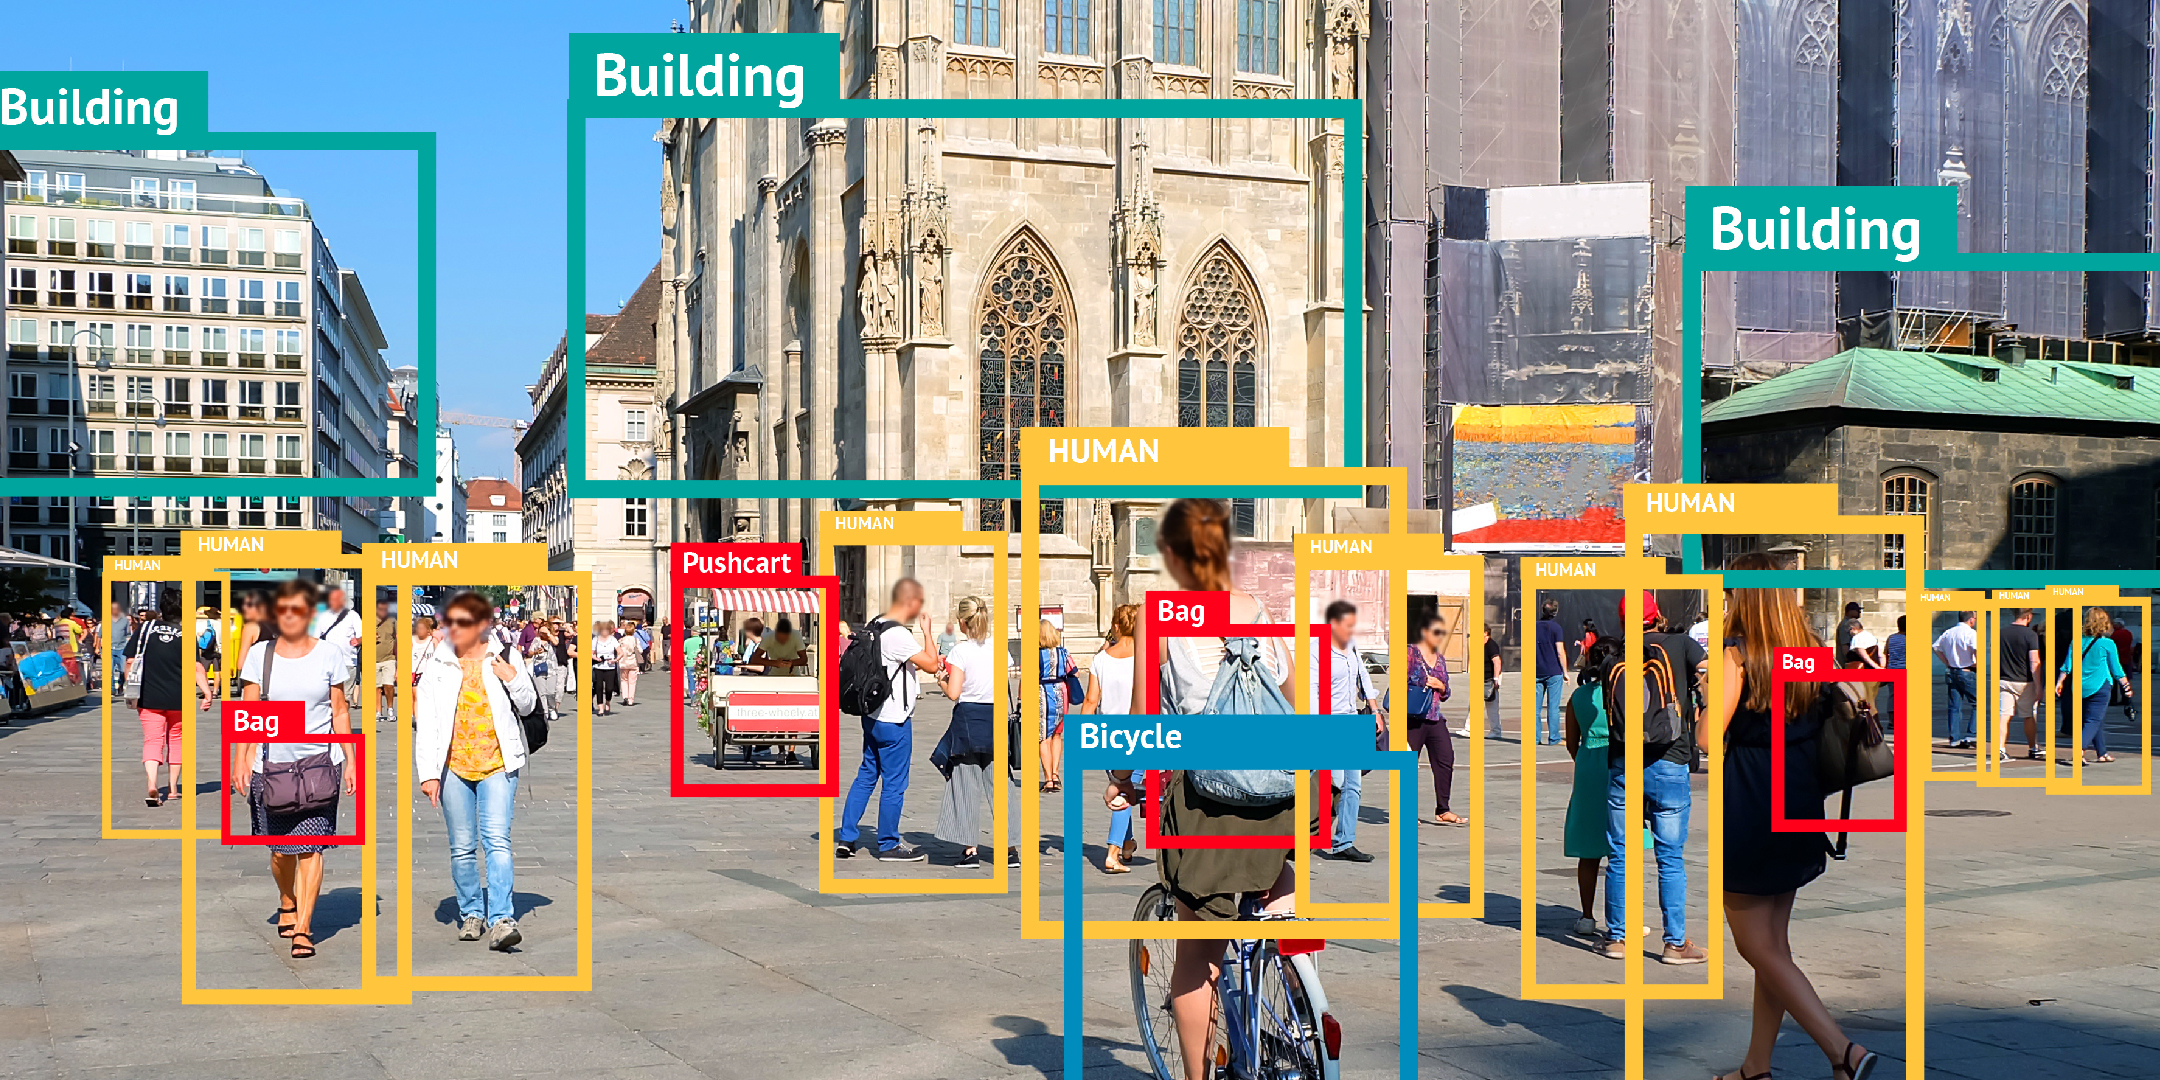
\includegraphics[width=0.9\linewidth]{Resources/Images/object_detection.jpg}
\caption{Object detection}
\label{fig:Object_detection}
\end{figure}

Object segmentation, also called semantic segmentation, seeks to create a per-pixel representation of the image in terms of the different objects or regions contained within(Fig. \ref{fig:Object_segmentation}). 

\begin{figure}[ht]
    \centering
    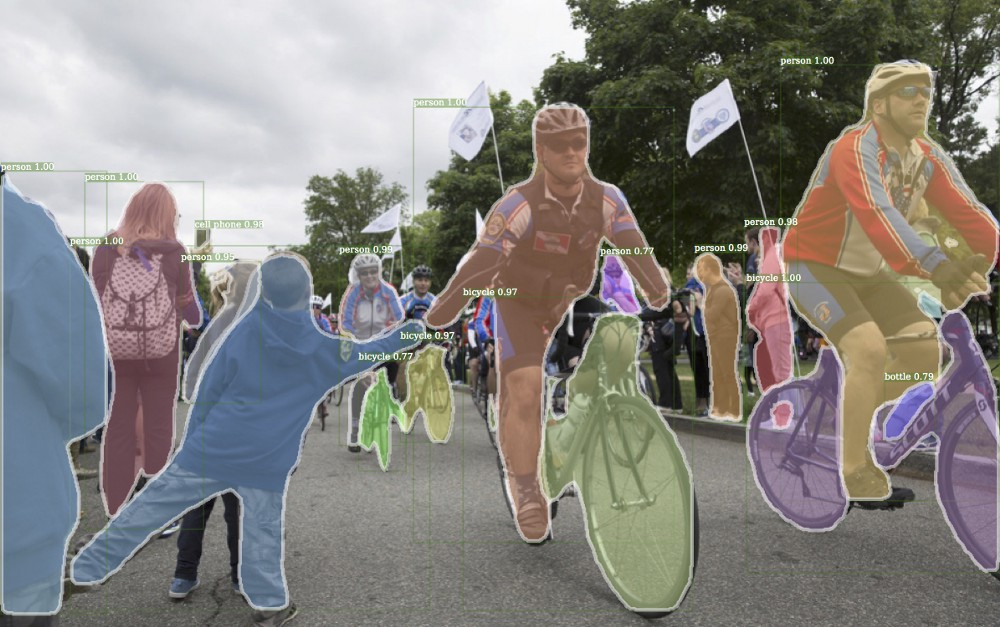
\includegraphics[width=0.8\linewidth]{Resources/Images/object_segmentation.jpg}
    \caption{Object segmentation}
    \label{fig:Object_segmentation}
    \end{figure}

\section{CNN: Convolutional Neural Networks}
\subsection{Origin}
Convolutional neural networks (CNNs) were inspired by the vision processing in living organisms. In 1968, Hubel and Wiesel published a paper\cite{hubel_wiesel_1968} identifying two basic cell types in the brain: simple and complex cells. According to their study, simple cells are specialized to maximize their output when they detect straight edges with particular orientations, while complex cells have a much larger field of detection, and their output is not sensitive to the exact position to the edges in their area. Hubel and Wiesel proposed the cascading model of these two cell types for use in pattern recognition. 

In 1980, Fukushima\cite{fukushima_1980} introduced the neocognitron, the basis of the two basic types of layers in CNNs: Convolutional layers, and Downsampling layers. The convolutional layers in a neural network are the equivalent to biological simple cell types, while the downsampling layers are the equivalent to the biological complex cell types, covering large patches of the previous layers. 

LeCunn et al. published in 1989\cite{LeCunn} their mythical Lenet paper, cementing the foundations of modern computer vision as we know it.

\subsection{Region based CNN: R-CNNs}
We fast-forward to 2013, passing several improvements to compute power and the concepts used in CNNs. Uijlings et al.\cite{uijlings_van} proposed a method of generating possible object locations for use in object recognition. This allowed the creation of Region-based CNNs (R-CNNs). 

R-CNNs are composed of four parts:
\begin{enumerate}
    \item Selective region search.
    \item Pre-trained CNN is placed in a truncated form before the output layer.
    \item Features and category of each proposed region are used to train a support vector machine (SVM) for the final object classification.
    \item The features and bounding box of the proposed regions are combined and used to train a linear regression model for ground-truth prediction.
\end{enumerate}

R-CNNs have the downside of being slower, even though they require the use of pre-trained CNNs. This stems from the forward computations required from the CNN to perform object detection on our proposed regions. 

\subsection{Fast R-CNNs}

Being extremely computationally expensive, R-CNN's bottleneck is the need to extract features for each proposed region independently. Since there is a disconnect between the network dedicated to region selection and feature extraction, and these regions overlap between each other, this feature extraction process results in a very high amount of repetitive and unnecessary computations. To solve this, in 2015  Girshick\cite{girshick_2015} proposes the Fast R-CNN architecture. 

Compared to previous architectures, Girshick introduces Region of Interest (RoI) pooling. Girshick uses the entire image as the original CNN input for feature extraction bypassing the region proposal method. The pipeline of fast R-CNN is as follow:

\begin{enumerate}
    \item Use the original image as the input for feature extraction, with a network trained to updatre the model parameters.
    \item With N proposed regions, features detected in the same shapes are extracted from these regions of interest. 
    \item The CNN output and RoIs are concatenated and to summarize the features extracted from each proposed region.
    \item A fully connected layer transforms the output shape to NxD, where D is determined by the model's design.
    \item Softmax regression is applied during class prediction, and the shape of the fully connected layer is transformed during bounding box prediction.
    \item Combining these two last changes to the shape of the layers, the class and bounding box are predict for each proposed region.
\end{enumerate}

\begin{figure*}[h!]    
    \centering
        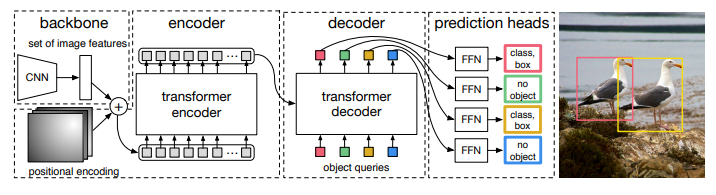
\includegraphics[width=0.9\textwidth]{Resources/Images/detr.png}
    \captionof{figure}{End-to-End Object Detection with Transformers (DETR) Pipeline}
    \label{fig:detr}
\end{figure*}

\subsection{Faster R-CNN}
The main issue with Fast R-CNNs is that it requires a high amount of region proposals generated in the initial selective search. This is computationally expensive and, as with the original R-CNN, results in unnecessary computations. 

The Faster R-CNN architecture, proposed by Shaoqin Ren, Kaiming He, Ross Girshick and Jian Sun\cite{ren_he_girshick_sun_2015} fixes this by replacing the selective search with a completely new neural network devoted solely to region proposal: a Region Proposal Network (RPN). 

The RPN is a fully convolutional network that predicts object bounding boxes and a confidence score. These bounding boxes are used as the input regions for the RoI pooling. The RPN is trained along the rest of the model, and can learn to generate high quality proposed regions, reducing the total number of regions that needs to be processed without affecting the precision of object detection negatively. 

\subsection{Mask R-CNN}
On March 2017, Kaiming He et al.\cite{he_gkioxari_dollár_girshick_2017} publish a second paper improving their architecture even further. Kaiming et al. extend the Faster R-CNN architecture following a similiar line of thought as they did with the RPN proposal: by adding a convolutional network after the RoI align to locate objects at a pixel level within the image. This aditional CNN runs parallel with the bounding box detection and class prediction branches. 

The added CNN is a feature pyramid network-styled CNN, consisting of a bottom-up pathway composed of any ConvNet/ResNet/VGG, that extracts features from raw images, a top-bottom pathway that generates a feature pyramid map, and two lateral convolution/addition operations between the corresponding levels of the two pathways. This FPN outperforms traditional ConvNets because it mantains features at various resolution scales. 

\subsection{Mesh R-CNN}
After mask R-CNNs, in 2019 Georgia Gkioxari, Jitendra Malik and Justin Johnson\cite{gkioxari_malik_johnson_2019} published a paper improving the pipeline to predict 3D shapes out of 2D images. They modify mask R-CNN in the same way the past two sections have done so: by introducing a new network to the pipeline. 

Gkioxari's team introduces a mesh prediction branch that triangle meshes predicting the shapes of the detected objects in three dimentions, following a pyramidal structure. They first predict coarse representations of the features, and then use these as inputs to a graph convolution network to refine them. These meshes are then put through ShapeNet where they are validated.

\section{End-to-End Object Detection with Transformers (DETR)}
The Facebook Research team has developed an object detection model, Detection with Transformers (DETR)\cite{carion_massa_synnaeve_usunier_kirillov_zagoruyko_2020}, that moves away from using R-CNN as the backbone of their pipeline, and instead utilize a transformer architecture. 

Seeing how previous approaches to object detection have to deal with post-processing of the output of their components due to duplicate (or irrelevant) predictions, the DETR team seeks to simplify the object detection pipeline by shifting to a direct set prediction model, with the objective of translating the improvements that transformer networks have brought upon the Natural Language Processing(NLP) scene into the computer vision scene.

As a baseline architecture proposal, DETR seeks to match the performance of Faster R-CNN pipelines. According to the DETR paper, the new transformer-based architecture(Fig. 3) generally outperforms Faster R-CNN, except when there are many small objects, where it obtains a worse performance.

\section{Week 3: Using pre-trained models on new datasets}

On week 3 of the M5 module, we are tasked to perform several experiments using 
the popular faster R-CNN and RetinaNet pre-trained models on two popular
datasets: KITTI-MOTS and MOTSChallenge. We will describe our results in the 
following sections.

\subsection{Task A}

For task A, we needed to take a look at the datasets we would use on the 
following experiments. The MOTSChallenge dataset involves a series of 
photographs of urban scenarios with several people on the frame,
identified with the "Pedestrian" class, and corresponding bounding boxes
for the ground truth annotations. The KITTI-MOTS dataset, augments the
challenge by adding a car category.

After looking into the annotations of these datasets, we notice that
the annotations need to be adapted to the notation that the COCO models
use to make them compatible and so that we can properly run inference on
these datasets using the pre-existing models.

\subsection{Task B: Qualitative analysis of Faster R-CNN and RetinaNet}

In this task, we use the pre-trained Faster R-CNN and RetinaNet on the
KITTI-MOTS validation set, and are asked to provide qualitative results.
We tested several of the models contained in the COCO model library, and 
ended up favouring the $"101\_32x8d\_FPN\_3x"$ model for 
RCNN (Fig. \ref{fig:r50r101}) and the $"R\_50\_FPN\_1x"$
model for RetinaNet (Fig. \ref{fig:r50retina}).

\begin{figure}[ht]
    \centering
    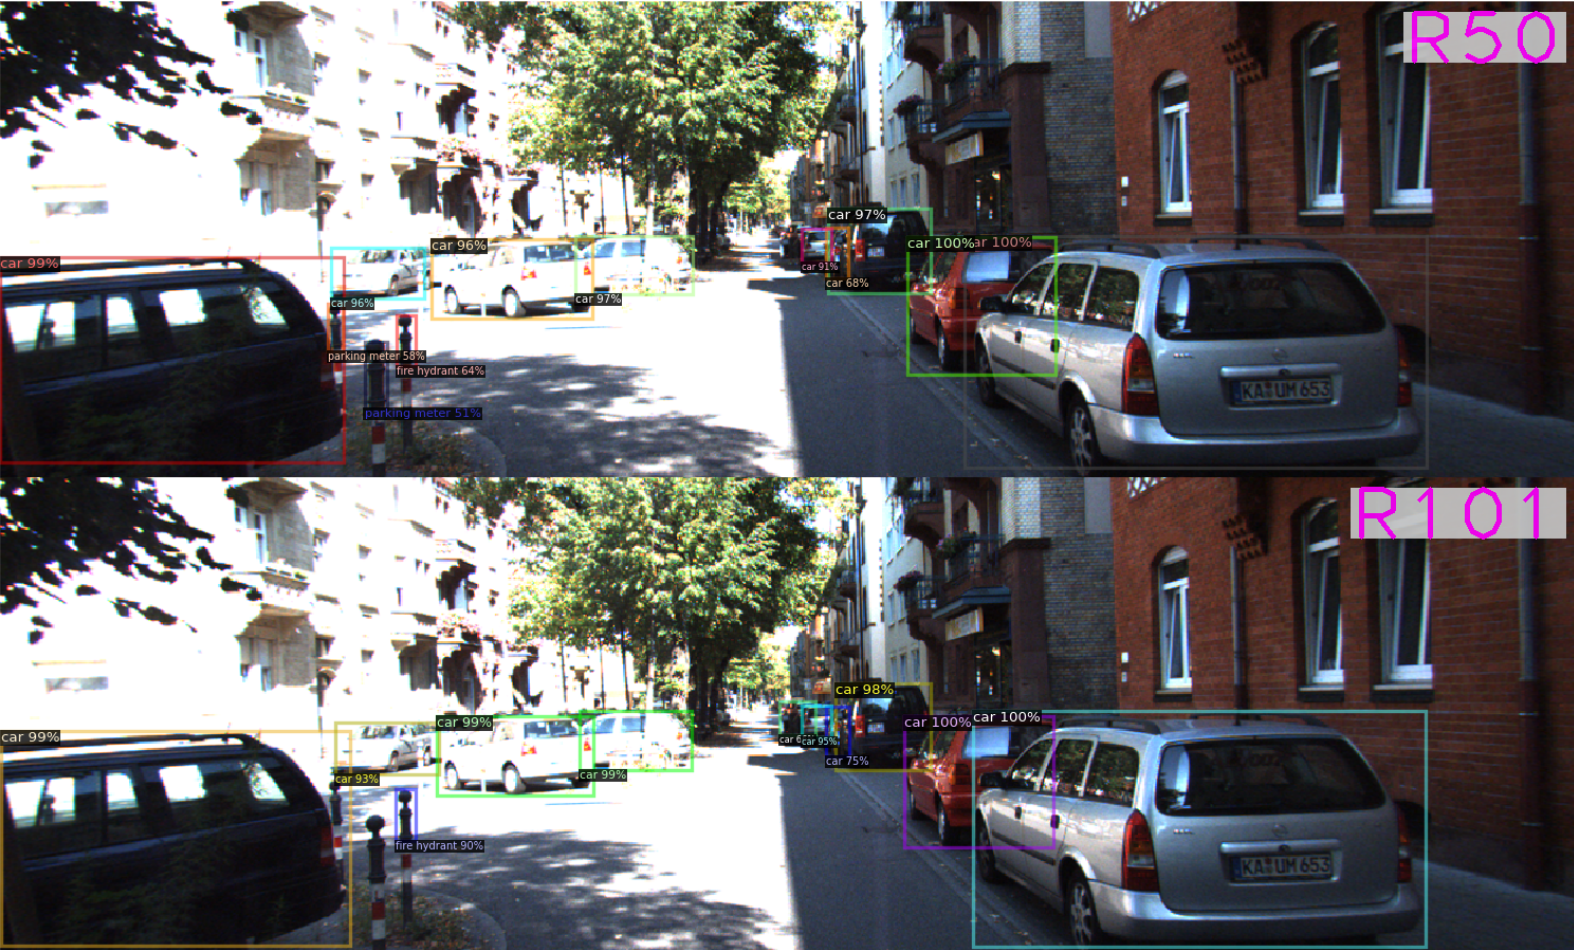
\includegraphics[width=0.8\linewidth]{Resources/Images/r50r101.png}
    \caption{RCNN samples.}
    \label{fig:r50r101}
    \end{figure}

\begin{figure}[ht]
    \centering
    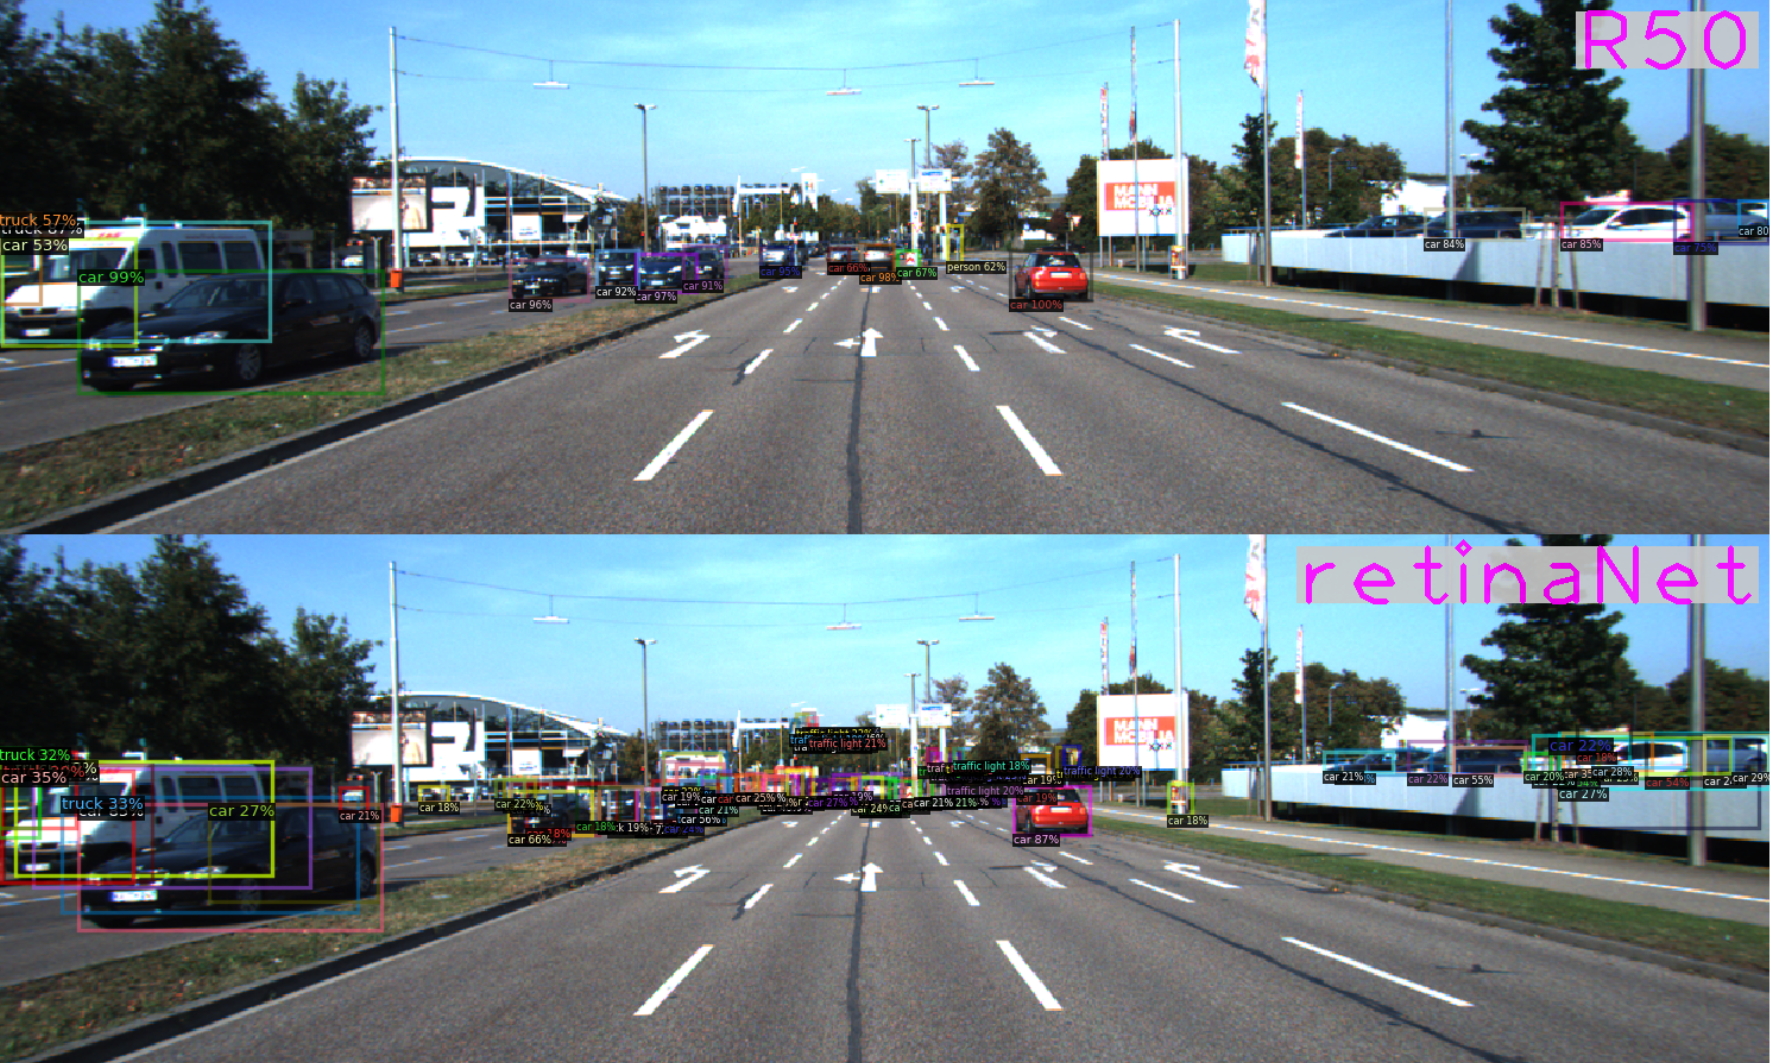
\includegraphics[width=0.8\linewidth]{Resources/Images/r50retina.png}
    \caption{RetinaNet samples.}
    \label{fig:r50retina}
    \end{figure}

\subsection{Task C: Quantitative analysis of pre-trained models.}

After last section's qualitative analysis, we are tasked with evaluating
quantitatively how these models perform on the validation of the KITTI-MOTS dataset. We used 
$AP_{(50)}$ metrics to compare the performance of the models, for both 
overall model performance and per-class performance (Table \ref{table:KITTI_Table1}.). 

\begin{table}[ht]
    \centering
    \begin{tabular}{|c || c | c|} 
        \hline
          & \textbf{R-CNN} & \textbf{RetinaNet} \\ [0.8ex] 
          \hline
         $AP_{(50)}$ & 0.415 & 0.461  \\ 
         \hline
         $AP_{(50)}$ Car & 0.576 & 0.553 \\
         \hline
         $AP_{(50)}$ Pedestrian & 0.456 & 0.397 \\
         \hline
    \end{tabular}
    \caption{\label{table:KITTI_Table1}Pre-trained $AP_{(50)}$ on KITTI-MOTS validation.}
\end{table}

Both models preform very well for Car objects, but the pedestrian class
represents a problem for their performance, especially on RetinaNet
which takes a larger nosedive in performance when trying to identify pedestrians
than RCNN.

\subsection{Task D: Quantitative analysis of models after training on new datasets.}

For task D we needed to train RCNN and RetinaNet on the datasets and provide
a quantitative analysis of the results. 

For training, validation and test splits, we used $60\%$ of the dataset as training, $20\%$
as validation, and $20\%$ as test. 
Our testing parameters were learning rate = {0.0001, 0.001, 0.01}, 
proposed regions = {32,64,128} at 1000 iterations.

We were able to collect data for the RCNN model 
(Table \ref{table:RCNN_Table_training}), but 
all our experiments for RetinaNet gave us much lower results when compared to the pre-trained
models used in the previous section, which in all probability means that we could not
implement our test cycle properly for RetinaNet. The results were beyond a -15\% performance
decrease, and were not included in the table. 

\begin{table}[ht]
    \centering
    \begin{tabular}{|c | c || c|} 
        \hline
        \textbf{LR} & \textbf{Regions} & \textbf{$AP_{(50)}$} \\ [0.8ex] 
            \hline
            0.0001 & 32 & 0.236 \\ 
            \hline
            0.0001 & 64 & 0.371\\ 
            \hline
            0.0001 & 128 & 0.394 \\ 
            \hline
            0.001 & 32 & 0.410\\ 
            \hline
            0.001 & 64 & 0.467\\ 
            \hline
            \textbf{0.001} & \textbf{128} & \textbf{0.572}\\ 
            \hline
            0.01 & 32 & 0.365\\ 
            \hline
            0.01 & 64 & 0.379\\ 
            \hline
            0.01 & 128 & 0.426\\ 
         \hline
    \end{tabular}
    \caption{\label{table:RCNN_Table_training}RCNN Training.}
\end{table}

\subsection{Task E: Evaluate trained model on KITTI-MOTS test set.}

For this last task, we took the best performing model of the last section and used
it on the official KITTI-MOTS test set. For this, the LR = 0.001, Regions=128 
trained model was selected. 


\begin{table}[ht]
    \centering
    \begin{tabular}{|c || c |} 
        \hline
          & \textbf{R-CNN}\\ [0.8ex] 
          \hline
         $AP_{(50)}$ & 0.331\\ 
         \hline
         $AP_{(50)}$ Car & 0.421\\
         \hline
         $AP_{(50)}$ Pedestrian & 0.367\\
         \hline
    \end{tabular}
    \caption{\label{table:KITTI-MOTS-FINAL}Final model $AP_{(50)}$ on KITTI-MOTS validation.}
\end{table}

As we can see in table \ref{table:KITTI-MOTS-FINAL}, our results are noticeably 
worse than the pre-trained model's results, even though we outperformed 
the pre-trained model on our train-validation-testing split. We suspect that this is due
to the images in the test set beneffiting from a higher region count for this model.

\printbibliography
\end{document}
